% !TeX spellcheck = en_US
\section{Joint Selection and Placement of Algorithms}
\label{sec:555_placement}
Besides novel algorithms for the detection and assessment of degradations common in \ac{UGV}, the assessment of video streams at runtime is a huge burden for centralized services.
A scalable solution is proposed, which leverages the resources of all recording devices and dynamically allocates quality assessment processes to the most appropriate devices.
A joint selection of an appropriate quality assessment algorithm and the placement of this algorithm on a device is proposed. 

Mobile video broadcasting includes several devices for the quality assessment.
The first node is the mobile device recording the stream.
Also, all close-by devices participate in the mobile broadcasting service can be used for running a quality assessment.
Besides the mobile devices, the receiving server, as well as other networking elements, can potentially run quality assessment algorithms.

The selection determines which algorithm meets given application requirements regarding precision and runtime.
These algorithms are classified into assessment types ($AT$), which not only include the recording quality assessment algorithms (proposed in the previous section), but also traditional video quality assessment metrics, that measure the effects of transport artifacts or compression.
\subsection{The Placement and Selection Component}
\label{sec:555_architecture}
Figure~\ref{fig:553_architecture} illustrates an overview on the \ac{PaSC}.
A common, decoupled component is available for the execution of the algorithms and the selection and placement decision.
\begin{figure}[!htb]
	\centering
	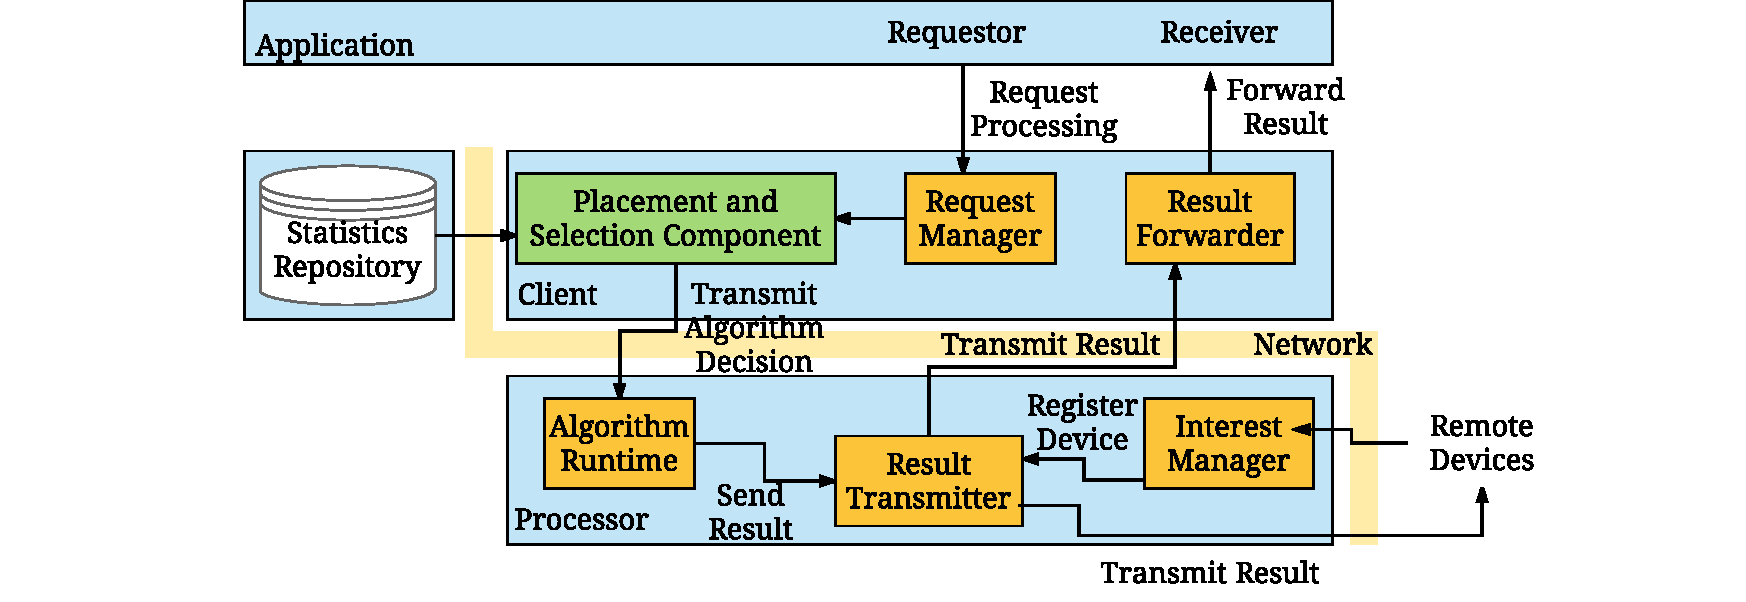
\includegraphics[width=\linewidth]{./gfx/550_QA/PASC_architecture}
	\caption[Subcomponents of the \ac{PaSC} running on each smart mobile device.]{Subcomponents of the \ac{PaSC} running on each smart mobile device for using the proposed scalable and adaptive quality assessment.}
	\label{fig:555_architecture}
\end{figure}
It consists of the following major building blocks: a statistics repository, an algorithm processor, and the algorithm client. Applications request the processing of algorithms and receives the results after completion. A client consists of the respective components to manage requests for algorithm execution from an application and the forwarding of the algorithm execution results. The core element of the client is the "Placement and Selection" component. As it is integrated into the client, each device individually makes the placement and selection decisions. Decision-making is based on statistics that devices regularly request from the repository. Processing of an algorithm happens on the devices (local processing), or relevant data is transmitted for remote processing to either other mobile devices or a server. In case a local device is selected, the computation can be started immediately on the device without any data transmission. 
For remote processing, a device receives the required sensor readings, e.g., the video. 
The respective components of the processor include the algorithm execution environment necessary for running the quality assessment algorithm, and components required for the result distribution.
Multiple devices, e.g., the local device and the server, can be interested in the quality assessment result.
Thus, a quality assessment request is handed to the interest manager module which allows any device to register for assessment results of a specific video stream. 
Once the result is available, all interested devices are informed.
 A mobile device may request a video quality assessment, and a composition server is informed about this assessment result.
After each execution of an algorithm on a device, the repository is informed of the current device state and statistics - including available and used energy, the runtime of the algorithm, and the available and used memory of the device. Coordination of statistics is achieved by using the repository block that builds a shared storage for statistics. 
\subsection{Steps for Selecting an Algorithm and a Processing Device}
The steps of selecting an algorithm and placing it on a device are illustrated in Figure~\ref{fig:555_steps}.
Once an application requests a quality assessment of a video stream, the device recording the video requests a list of the devices available for processing and the related statistics from the repository.

All available devices and the subset of the algorithms are then considered in the selection, as described in Section~\ref{sec:550_design_quality_selection}.

A preprocessing step allows algorithms to determine their runtime characteristics on any device.
Usually, this preprocessing requires the execution of algorithms on a device before it runs the \ac{PaSC}, which is unfeasible in a real deployment.
Thus, devices are categorized into "device types" to reduce the preprocessing effort.
A "device type" can be the specific model of a smart mobile device; or, as in our case, a categorization according to high-end servers, low-end, medium-end and high-end smartphones.
A device is classified when it starts using the \ac{PaSC}.
The runtime measurements of other devices of the same "device type" can then be used for a joining device.
In this thesis, the devices are classified using the results of the benchmark databases Vellamo\footnote{Qualcomm Vellamo Metal Benchmark; Visited on: 10/09/2016} and AnTuTu benchmarks\footnote{AnTuTu Benchmark, \url{http://www.antutu.com/en/index.shtml}; Visited on: 10/09/2016} (see Section~\ref{sec:557_eval_setup}).

\begin{figure}[!htb]
\centering
    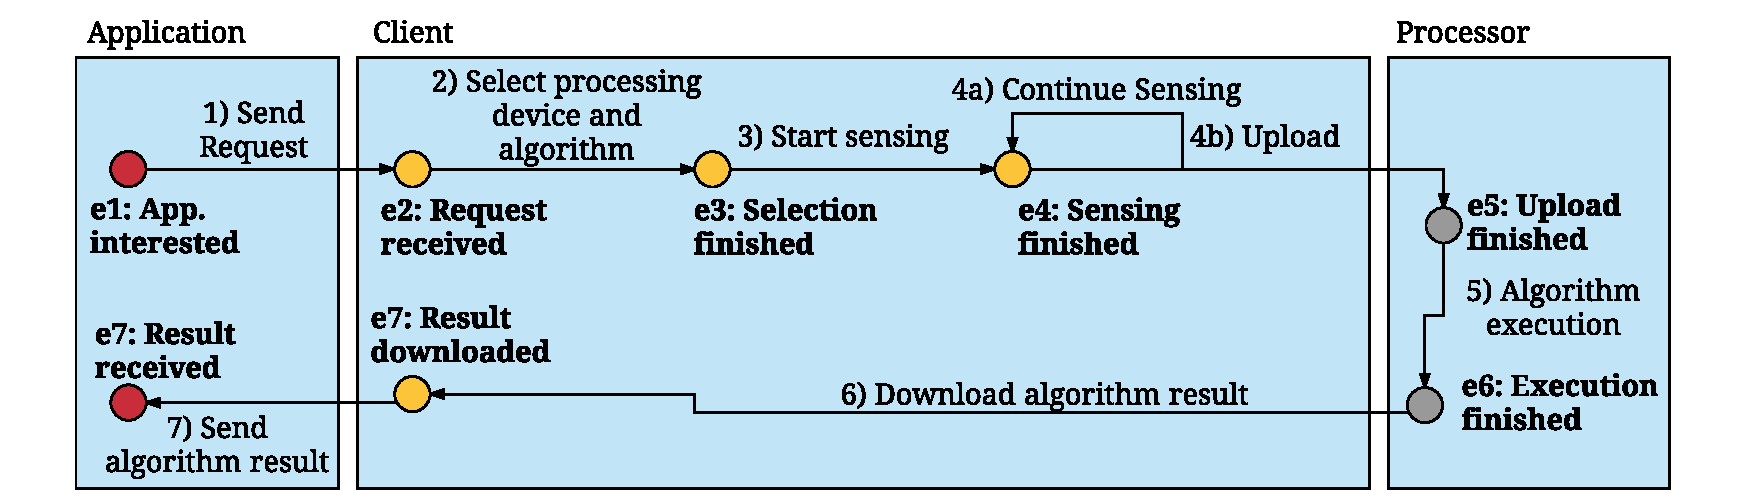
\includegraphics[width=\linewidth]{gfx/550_QA/fromRequestToReceive}
    \caption{\ac{PaSC}: From sensor values to the measured results.}
    \label{fig:555_steps}
\end{figure}
Figure~\ref{fig:555_steps} depicts the steps and occurring events in this component for requesting (e1), selection, and placement of an algorithm (e3 - e5), and the processing of the algorithm (e6).
The selection and placement decision-making are explained in the next section.
%==================================================================
\subsection{Selection and Placement Algorithm}
\label{sec:550_design_quality_selection}
The goal is to select one algorithm $a \in S_{AT}(a_{AT,1} ... a_{AT,n})$ to be processed by a device $d \in D(d_{1}...d_{m})$.
$S_{AT}$ represents the subset of algorithms that analyze a specific set of degradations, i.e., recording quality, video quality, or audio quality assessment.
The selection of an algorithm and a processing device relies on a comparison of the utility $u_{a}$ and the costs $c_{a,d}$ for processing $a$ on $d$.
For all algorithms and all devices, the idea is to maximize the difference of utility ($u_{a}$) to costs ($c_{a,d}$):
\begin{equation}
max \sum_{a=0}^{o} \sum_{d=0}^{p} (u_{a} - c_{a,d}) * x_{a,d}
\end{equation}
It determines the maximum utility-to-cost proportion for executing an algorithm $a$ on a device $d$.
The result is in the range $[-1,1]$ as both $u_{a}$ and $c_{a,d}$ are normalized to $[0, 1]$.

To ensure that exactly one algorithm $a$ is processed on one device $d$ the following condition must hold:
\begin{equation}
\sum_{a=0}^{o} \sum_{d=0}^{p} x_{a,d} = 1
\end{equation}
Here, $x_{a,d}$, a binary value, shows if $a$ is executed on $d$ where $x_{a,d} \in \{0,1\}$.
Practically speaking, we iterate over all combinations of running each algorithm on any device and determine the best combination.

The utility ($u_{a}$) is represented by the precision of an algorithm and is described in our case as its precision.
The metric is device-independent as we assume deterministic algorithms. 
The cost statistics include the \textit{processing time} ($\tilde{t}(a, d)$), \textit{energy} ($\tilde{e}(a, d)$), \textit{memory} ($\tilde{m}(a, d)$), and \textit{data traffic} ($\tilde{dt}(a, d)$) spent by an algorithm.
The costs $c(a, d)$ are calculated by:
\begin{equation}				 
w_t * \frac{\tilde{t}(a, d)}{N_c} + w_e * \frac{\tilde{e}(a, d)}{N_c} + w_m * \frac{\tilde{m}(a, d)}{N_c} + w_{dt} * \frac{\tilde{dt}(a, d)}{N_c}
\end{equation}
Furthermore, $c(a, d)$ uses $N_c = 4$ to normalize results to a range between $[0,1]$.
$N_c$ represents the number of different cost components of $c(a, d)$.
Both utility ($u_{a}$) and costs ($c(a, d)$) are normalized to $[0,1]$.
Here, we define the $\tilde{t}(a, d)$ to be the normalized scalar in respect to the maximum runtime measured for an algorithm $a$ on any available device in $D(d_{1}...d_{m})$.
For the execution time it results in:
\begin{equation}
\tilde{t}(a, d) = \frac{\overline{t(a, d)}}{t(a_{AT,max})} 
\end{equation}
$\tilde{t}(a, d)$ is calculated as the average of all completed runs of algorithm $a$ on a device $d$ in comparison to the maximum runtime ($t(a_{AT,max})$) of algorithms in $S_{AT}$ and the device set $D$.
$t(a_{AT,max})$ represents the maximum runtime of the slowest running algorithm in the set $S_{AT}$: $a_{AT,max} = argmax_{a}(t(a, d))$. 
The remaining cost components have similar formulas and are thus not discussed in detail.

The costs can be adjusted by the weights $w_t$, $w_e$, $w_m$ and $w_{dt}$, which indicate the relevance of different cost components where a value of zero represents no relevance and a value of 1 represents the maximum relevance for the selection of an algorithm: $w_t \in [0,1]$, $w_e \in [0,1]$, $w_m \in [0,1]$ and $w_{dt} \in [0,1]$.
These weights can be set by application designers to adjust the impact of certain cost components on the selection.
E.g., for applications where the caused data traffic is rather negligible the weight $w_{dt}$ can be set close to 0. 
For the proposed video composition scenarios, the weights are set according to $w_t = 1$, $w_e = 1$, $w_m = 0.5$ and $w_{dt} = 0.5$ in order to favor algorithms with short processing times in the selection process.
\subsection{Algorithm Implementation to Support the PaSC}
PaSC is available for the Java Runtime Environment and Android\footnote{Details on the implementation are available from our repository Chapter~\ref{app:repository}.}.
Thus, all algorithms are realized using Java (auxiliary-sensor based algorithms) or are encapsulated by the Java Native Code injecting C code (video-based algorithms).
Video-based algorithms leverage \ac{JNA} as the algorithms implemented using C run significantly faster for mobile devices. 
The speed-up for a LG Nexus 5 is between 2.2 to 17.8 times.
The \ac{PaSC} assumes that the algorithm implementations are available on all devices.
The integration of a new algorithm requires an update of the \ac{PaSC}. 
A solution to this issue, which is not investigated in this thesis, is the migration of code at runtime. 
Related research provides frameworks that can be used to support code migration~\cite{Aitenbichler2007}.

Each device reports the execution time, a sample on the used device memory, a measurement of the energy drain, and an estimation on the caused data traffic after an algorithm run is completed.
The energy drain is only measured for mobile devices.
We leverage the implementation of the PowerTutor tool provided by the University of Michigan\footnote{http://ziyang.eecs.umich.edu/projects/powertutor/; Visited on: 10/13/2016} to estimate the energy drain caused by an algorithm execution.
The usage of PowerTutor for measuring the energy consumption of video-based algorithm has shown to provide a sufficient reliability~\cite{Ganiyu2012}.
The remaining statistics (processing time, data traffic and memory) are implemented using Java and \ac{OS} functions.